\documentclass[english,serif,mathserif,usenames,dvipsnames]{beamer}
\usetheme[informal]{gc3}

\usepackage[T1]{fontenc}
\usepackage[utf8]{inputenc}
\usepackage{babel}

%% This is optional: it adds a few commands and environment we
%% regularly use in our slide sets
\usepackage{gc3}

\begin{document}

%% Optional Argument in [Brackets]: Short Title for Footline
\title[Lisp]{A quick introduction to Lisp}
\subtitle{(by a dummy)}
\author{Pierre-Yves Dupont}
\date{\today}

%% Makes the title slide
\maketitle


\begin{frame}[fragile,fragile]{Remark: Use Numpy vectors (implicit vectorization during operation on vectors)}
	Much faster: why?
    
	\begin{itemize}
    \item<1-> Operations faster in NumPy (\emph{C} libraries)
    \item<2-> Operations on vectors possible
    \end{itemize}

\end{frame}


\begin{frame}[fragile,fragile]{Remark: Use Numpy vectors (implicit vectorization during operation on vectors)}
	Simple python code:
    
    \begin{python}
N = 1e4
a = numpy.random.random((N))
b = numpy.random.random((N))

c = numpy.zeros((N,N))

^\HL{for i in range(len(a)):}^
^\HL{  for j in range(len(b)):}^
^\HL{    c[i] = a[i] + b[j]}^
    \end{python}
  
  \only<2->{Execution in $\approx 1.23$ minutes} 

\end{frame}

\begin{frame}[fragile,fragile]{Remark: Use Numpy vectors (implicit vectorization during operation on vectors)}
	Should be written:
    
    \begin{python}
N = 1e4
a = numpy.random.random((N))
b = numpy.random.random((N))

c = numpy.zeros((N,N))# not mandatory

^\HL{c = a + b}^
    \end{python}
  
  \only<2->{Execution in less than a second!}

\end{frame}

\begin{frame}[fragile,fragile]{Remark: Use Numpy vectors (implicit vectorization during operation on vectors)}
	
    Conclusion:\\
    You don't necessarily need Lisp, C++, Java, \dots to build an efficient code

\end{frame}

\begin{frame}[fragile,fragile]{Introduction to Lisp}
	\begin{itemize}[<+->]
    \item Short introduction
    \item Some myths and facts
    \item What Lisp offers
    \end{itemize}
\end{frame}

\begin{frame}[fragile,fragile]{Some history}
	\begin{itemize}[<+->]
    \item[1958] Lisp, Lisp 1.5 (John McCarthy - AI pope): LISP = A LISt Processing language. One year after Fortran 
    \item[1962] First Lisp compiler (Maclisp)
    \item[1975] Scheme (one of the two main dialects of Lisp)
    \item[1984] Common Lisp (1994 for the ANSI version)
    \item[2007] Clojure (Lisp over a VM (Python , Java, Ruby) or compiled to JS - used as a macro system)
    \end{itemize}
\end{frame}

\begin{frame}[fragile,fragile]{LISP}
	\begin{itemize}[<+->]
	\item Functional programming object: each expression in LISP is a function that returns a value. Ex: numbers is a function returning itself\dots
	\item Object layer (CLOS)
	\item Polish prefix notation: \emph{(+ 1 2)} and not \emph{1 + 2}
	\item Interpretive language: LISP programs are interpreted by the LISP interpreter (example: \emph{clisp}). Compilers exist (much faster)
	\item Most of AI programs in US are written in LISP. (PROLOG for Europe)
	\item Native (and efficient) Tree Data Structure
	\item Source code as a data structure: flexible macro system
	\item ASDF (Another System Definition Facility) libraries manager (Gem, CPAN)
    \end{itemize}
\end{frame}


\begin{frame}[fragile,fragile]{Example: "Hello world"}
	\begin{block}{Python}
    	\begin{python}
	    print "Hello world" #python 2.x
	    print("Hello world")#python 3.x
	    \end{python}
	\end{block}

    \begin{block}{Lisp}
		\begin{lisp}
	    (print "Hello world")
	    \end{lisp}
    \end{block}
\end{frame}


\begin{frame}[fragile,fragile]{Example: Factorial (recursive)}
	\begin{block}{Python}
    	\begin{python}
def factorial(n):
    if n <= 1: 
        return 1
    return n * factorial(n-1)
	    \end{python}
	\end{block}

    \begin{block}{Lisp}
		\begin{lisp}
(defun factorial (n)
   (if (<= n 1)
       1
       (* n (factorial (- n 1)))
   )
)
	    \end{lisp}
    \end{block}
\end{frame}

\begin{frame}[fragile,fragile]{Myths}
	\only<1-2>{Myth: LISP = Lost In Stupid Parenthesis?}
	\only<2-2>{Fact: Question of point of view\dots}
	\only<3>{\centering{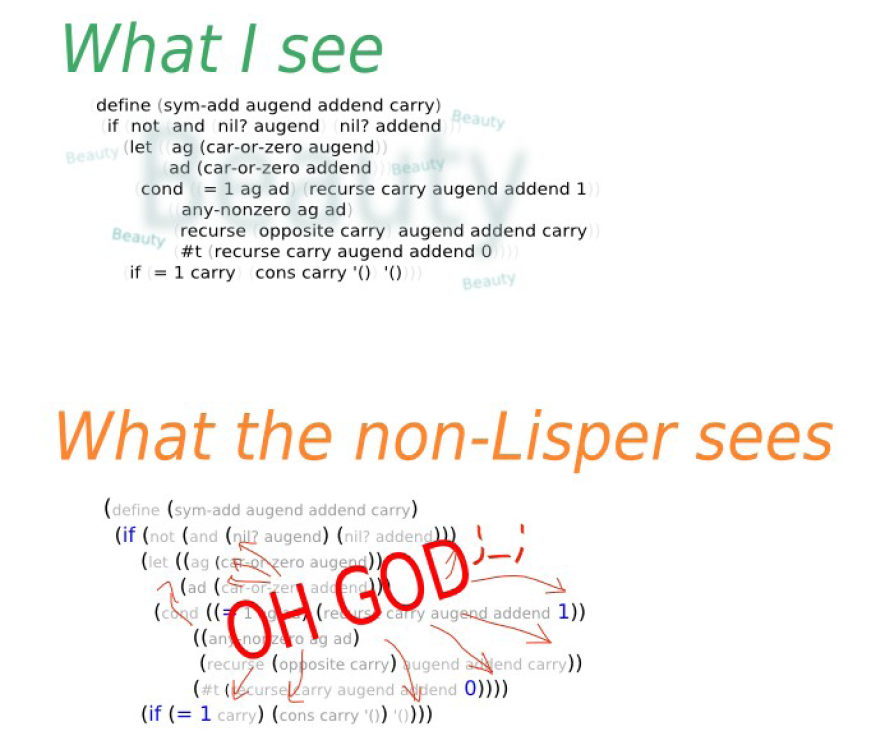
\includegraphics[width=9cm]{parenthesis.png}}}
\end{frame}

\begin{frame}[fragile,fragile]{Myths}
	\only<1->{Myth: There are no libraries in Lisp\\}
	\only<2->{Fact: About 2000 libraries in QuickLisp\\}
	\only<3->{vs. about 27,500 in PyPI\dots}
\end{frame}

\begin{frame}[fragile,fragile]{Myths}
	\only<1->{Myth: Lisp is slow\\}
	\only<2->{Fact: Fastest dynamic language. Can be faster than Java or C\\}
	\only<3->{K Nucleotide benchmark: 104 sec for Lisp vs. 923 for Java\\ \url{benchmarksgame.alioth.debian.org/u32q/lisp.php}}
\end{frame}

\begin{frame}[fragile,fragile]{Exact computation of fractions}
	\begin{lisp}
[1]> (/ 1 3)
1/3
[2]> (* (/ 1 3) 10)
10/3
[3]> (* (* (/ 1 3) 10) 1/2)
5/3	    
[4]> (format t "~d" x)
1/3
[5]> (format t "~f" x)
0.33333334

	\end{lisp}
\end{frame}

\begin{frame}[fragile,fragile]{Macros}
\begin{itemize}
\item A macro is a piece of code expanded at compile-time in a resulting form that is compiled by the compiler
\item macros do not evaluate their arguments
\item nightmare to debug!
\end{itemize}
\end{frame}

\begin{frame}[fragile,fragile]{Macros}
\begin{itemize}
\item Code generator
\item Tool for abstraction
\item Need a compilation step by definition
\item Used for:
\begin{itemize}
\item code generation, including objects (AI)
\item creation of new operators (ex: until)
\item parser generation
\item execution of code at compilation time
\end{itemize}
\end{itemize}
\end{frame}

\begin{frame}[fragile,fragile]{Creation of an operator using macros}
Unless operator:\\
\begin{lisp}
(defmacro unless* (test expr)
	`(if, test nil, expr))

(unless* nil(println "This should print"))
(unless* t(println "This shouldn't print"))
\end{lisp}
\end{frame}

\begin{frame}[fragile,fragile]{(Useless but simple) macro example}
Iteration on Prime Numbers:\\
Utility functions
\begin{lisp}
(defun primep (number)
  (when (> number 1)
    (loop for fac from 2 to (isqrt number) 
    	never (zerop (mod number fac)))))

(defun next-prime (number)
  (loop for n from number when (primep n) return n))
\end{lisp
You want to be able to write:
\begin{lisp}
(do-primes (p 0 19)
  (format t "~d " p))
\end{lisp}
\end{frame}

\begin{frame}[fragile,fragile]{(Useless but simple) macro example}
Iteration on Prime Numbers:\\
The macro
\begin{lisp}
(defmacro do-primes ((var start end) &body body)
  `(do ((,var (next-prime ,start) 
  	(next-prime (1+ ,var))))
       ((> ,var ,end))
     ,@body))
\end{lisp}

\begin{lisp}
(do-primes (p 0 19)
  (format t "~d " p))
  
2 3 5 7 11 13 17 19 
\end{lisp}
\end{frame}

\begin{frame}[fragile,fragile]{Strength of Lisp}
	\begin{itemize}
	\item efficient to work on lists, including linked lists and hash maps (sorts, pivots, accession to elements,\dots) because Lisp implementation is based on lists and linked lists 
	\item pattern matching (and regular expression)
	\item definition of new mini-languages: DSL
	\item metaprogramming: computer programs writing or manipulating other programs (or themselves) as data
	\end{itemize}
\end{frame}

\begin{frame}[fragile,fragile]{To go further}
\begin{itemize}
\item \href{http://gigamonkeys.com/book/}{Practical Common Lisp }
\item \href{http://kuomarc.wordpress.com/2012/01/27/why-i-love-common-lisp-and-hate-java/}{Why I love Common Lisp and hate Java}
\item \href{http://www.cs.sfu.ca/CourseCentral/310/pwfong/Lisp/1/tutorial1.html}{Lisp tutorial}
\end{itemize}
\end{frame}

\begin{frame}[fragile,fragile]{Bonus: How to choose a programming language?}
\begin{enumerate}[<+->]
\item Figure out what works for the team/company: \only<1>{Media: Ruby, PHP, JS, Java; Enterprise: Java, C\#; Research: Scala (simplified Java), C++, Erlang, Java and Python}
\item Find out what works in context
\item Consider ease of learning and use for computer programming languages
\item Evaluate the availability of tools (or libraries) for each of your potential computer programming languages
\item Look at cross-platform ability
\item Determine the ease of server-side and client-side scripting
\end{enumerate}
\tiny{\href{http://www.wikihow.com/Choose-a-Programming-Language}{Choose a Programming Language}}
\end{frame}

\end{document}

%%% Local Variables:
%%% mode: latex
%%% TeX-master: t
%%% End: